%\documentclass[fleqn]{book}
\documentclass[11pt]{amsbook}

\usepackage[turkish]{babel}

%\usepackage{../HBSuerDemir}	% ------------------------
\usepackage{../Ceyhun}	% ------------------------
\usepackage{../amsTurkish}

\begin{document}


% ++++++++++++++++++++++++++++++++++++++
\hPage{203}
% ++++++++++++++++++++++++++++++++++++++

\begin{figure}[htbp] \begin{center}
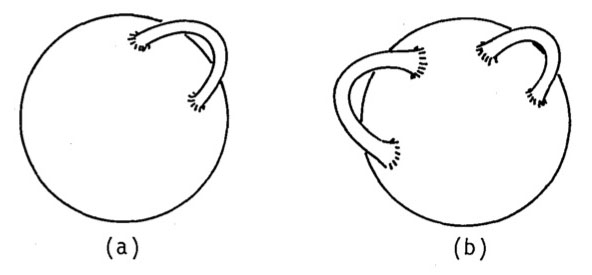
\includegraphics[width=1\textwidth]{images/ceyhun-203-fig01}
\caption{
Bir ve iki tutamaklı yuvarlaklar.
}
\label{fig:SuerDemirCovers} \end{center}
\end{figure}

\begin{figure}[htbp] \begin{center}
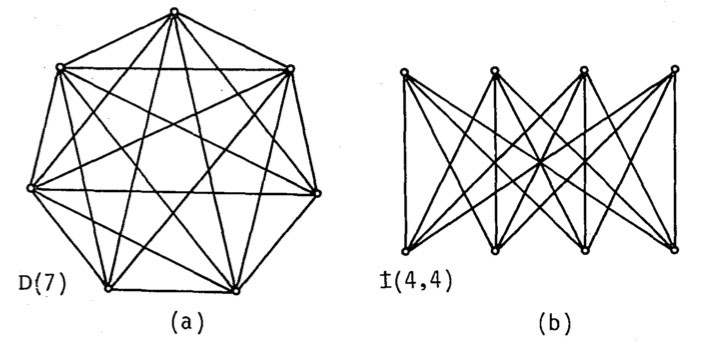
\includegraphics[width=1\textwidth]{images/ceyhun-203-fig02}
\caption{
Düzleme çizilemeyen $D(7)$ ve $İ(4,4)$ çizgeleri.
}
\label{fig:SuerDemirCovers} \end{center}
\end{figure}

\par 

tutamaklı yuvarlağın üzerine çizebiliriz. Böylesine bir yüzeyin, Şekil 4.2.8'de gösterildiği




\end{document}